\documentclass[12pt,italian]{report}
\usepackage{tesi}

\usepackage[a4paper]{geometry}		% Formato del foglio
\usepackage[italian]{babel}			% Supporto per l'italiano
\usepackage[utf8]{inputenc}			% Supporto per UTF-8
\usepackage[a-1b]{pdfx}				% File conforme allo standard PDF-A (obbligatorio per la consegna)
\usepackage{eso-pic}

\usepackage{graphicx}				% Funzioni avanzate per le immagini
\usepackage{hologo}					% Bibtex logo with \hologo{BibTeX}
%\usepackage{epsfig}				% Permette immagini in EPS
%\usepackage{xcolor}				% Gestione avanzata dei colori
\usepackage{amssymb,amsmath,amsthm} % Simboli matematici
\usepackage{listings}				% Scrittura di codice
\usepackage{url}					% Visualizza e rendere interattii gli URL
\usepackage{hyperref}				% Rende interattivi i collegamenti interni
\usepackage{tikz}                   % Permette di disegnare inline
\usepackage{import}
\usepackage{float}
\usepackage{xstring}                % Permette di usare la funzione \IfInteger
\usepackage{array}                  % Permette di usare colonne "m" dentro table
\usepackage{riassunto}              % Personalizzazioni per il riassunto
\graphicspath{{immagini/}}

\begin{document}

\chapter*{Riassunto elaborato}

\AddToShipoutPicture*
    {\put(450,593){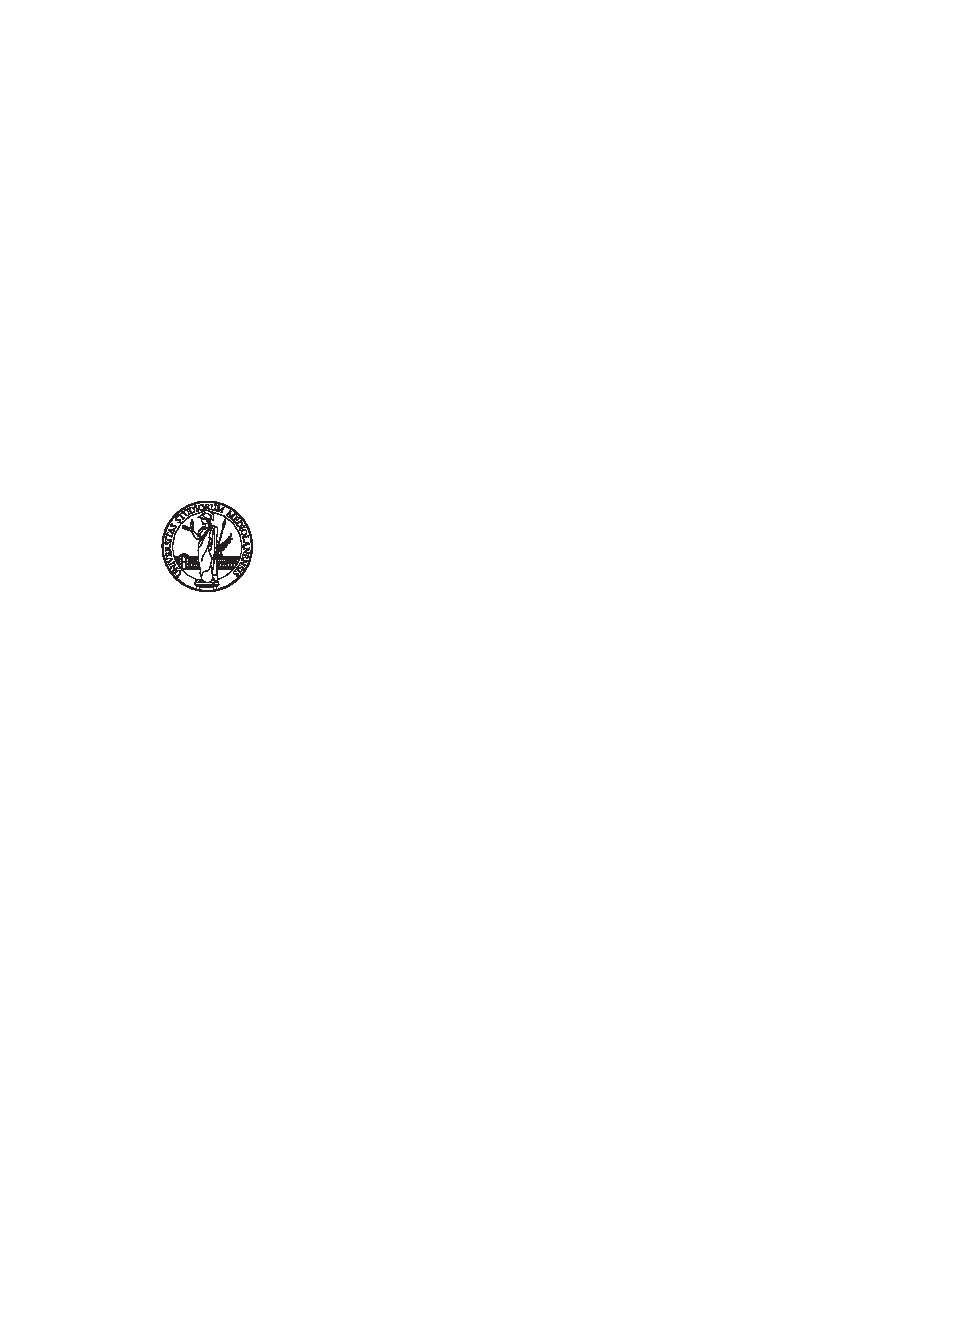
\includegraphics[width=23mm,height=23mm]{immagini/unimi}}}

\textbf{Titolo elaborato:} Sicurezza Hardware in Ambienti Virtualizzati Tramite un Passthrough TEE tra QEMU e Linux

\vskip 0.8 cm

L'aumento dei servizi che vengono richiesti dai moderni dispositivi di
computazione ha creato un quesito: l'aspetto di sicurezza è diventato più
importante di prima, ma con la maggiore complessità di tali sistemi aumenta
anche la superficie di attacco.
Rimuovere funzionalità dal sistema principale per renderlo più sicuro non
è accettabile, ma è possibile isolare i servizi critici dal punto di vista
della sicurezza in ambienti di computazione separati.

Questa è l'idea alla base dei \textit{Trusted Execution Environment(TEE)},
creare un ambiente di computazione nel processore isolato dal resto del
mondo non sicuro e dedicato solamente a quei software con requisiti di
sicurezza stringenti.
Normalmente un software è completamente esposto a tutto il codice
presente nel sistema con un livello di privilegio superiore;
i TEE si separano da questa gerarchia isolando la propria memoria e i propri
dati dal resto del sistema affidandosi a una base hardware e software
molto piccola.

I TEE sono molto diffusi in ambito mobile, dove vengono utilizzati per
isolare servizi come l'autenticazione di dati biometrici oppure la gestione
di pagamenti digitali, ma inizia a esserci un crescente interesse al loro
uso anche in ambito cloud per motivi di maggiore sicurezza, normative dati e 
per la possibilità di accertarsi che il software in esecuzione sul server
sia effettivamente quello che ci si aspetta.

Gli sforzi finora fatti in questo ambito sono stati rivolti verso permettere
ai clienti di portare i propri interi TEE; questa soluzione offre una grande
flessibilità ma implica anche uno sforzo significativo da parte del cliente
di gestire il proprio TEE, che per definizione è completamente inaccessibile
al vendor del cloud.

Le soluzioni oggi disponibili sul mercato sono esclusivamente per
l'architettura x86\_64 e implicano un lock-in rispetto le tecnologie
proprietarie di Intel e AMD.

Questa tesi si propone di studiare un modello alternativo dove il provider
di servizi cloud offre un TEE con dei servizi pre-installati offerti ai
clienti
Questo modello, seppur meno flessibile, è più semplice per il cliente e non
è in contrasto con il modello precedente, offrendo un'alternativa
ai clienti che non vogliono gestire il proprio TEE.
Inoltre, con la standardizzazione dell'interfaccia esterna TEE da parte di
dell'organizzazione GlobalPlatform, è anche possibile evitare il lock-in
rispetto a un TEE specifico o a una architettura in particolare.

Per dimostrare la fattibilità di questo modello abbiamo sviluppato un
prototipo estendendo l'hypervisor QEMU e utilizzando il sottosistema
TEE di Linux.
Questo ha richiesto di progettare un device virtuale, con un relativo protocollo
di comunicazione a messaggi, che permetta la comunicazione tra una macchina
virtuale e il TEE della macchina host, oltre a sviluppare un driver Linux
per questo nuovo device.

Per verificare la correttezza del nostro prototipo abbiamo integrato
\textit{xtest} con il nostro prototipo, una test suite di circa 10000 test
utilizzati da \textit{TrustedFirmware} per verificare la correttezza del
TEE open-source OP-TEE.
Grazie a questa test suite, abbiamo inoltre misurato le performance: 
seppur non eccezionali, anche se accettabili per determinati contesti,
abbiamo identificato che le cause sono problemi puramente ingegneristici e
non dovuti a limitazioni intrinseche del modello operativo.

Questo non è che un primo passo verso l'integrazione di tale modello in un
ambiente cloud.
Rimangono infatti da risolvere alcuni problemi, ad esempio come gestire
lo spostamento delle computazioni 
Sarebbe inoltre interessante integrare questo modello in un hypervisor di
tipo 1 e verificare il suo funzionamento in un ambiente reale. 

In conclusione, crediamo che il nostro prototipo sia fattibile e che possa
essere un buon punto di partenza per un'implementazione completa.


\bibliographystyle{unsrt}
\bibliography{bibliografia}
\addcontentsline{toc}{chapter}{Bibliografia}

\end{document}
